\documentclass[../Thesis.tex]{subfiles}
\graphicspath{{\subfix{../figures/}}}
\begin{document}

\chapter{Data}\label{chap:data}
In this chapter, we will introduce the pharmaceutical production data, that we shall later use to infer a causal structure pertaining different parts of the production system. In particular, as we are interested in the duration and amount of produced substance during the production flow, these are highly relevant attributes of the processes that make up the production. Hence, we will start this chapter with an overview of the production system, how the observations are structured and created to begin with. For the rest of the chapter, we will concern ourselves with analysis of the production system such as basic statistics, incomplete or wrongly labelled observations and initial observations about codependency (which is very relevant when studying causality).

The observations that we will ultimately use for the causal study is simulated by \cite{benchmark-model-to-generate-batch-process-data}. However, before diving into how these simulations were carried out, we present the overall structure of the simulated observations and the production system they are supposed to originate from. Namely, a set of $6$ cycles, where each cycle consists of a set of batches executed one by one. Thus, as cycle is simply a notion for multiple batches that are executed in continuation of each other. In particular, different settings for the simulation of each cycle have been used to encompass multiple scenarios of how the production system can function. We note that although the cycles are generated from different settings, they are still representative of the same production system. Hence, we shall later combine observations from all cycles.

A batch refers to a collection of processes/unit $\mathcal{U}$ that need to be executed in some order to produce a product. In particular, for this simulation study, each batch is a collection of the processes depicted in \autoref{fig:Cycle and process structure}.
\begin{figure}[ht]
    \centering
    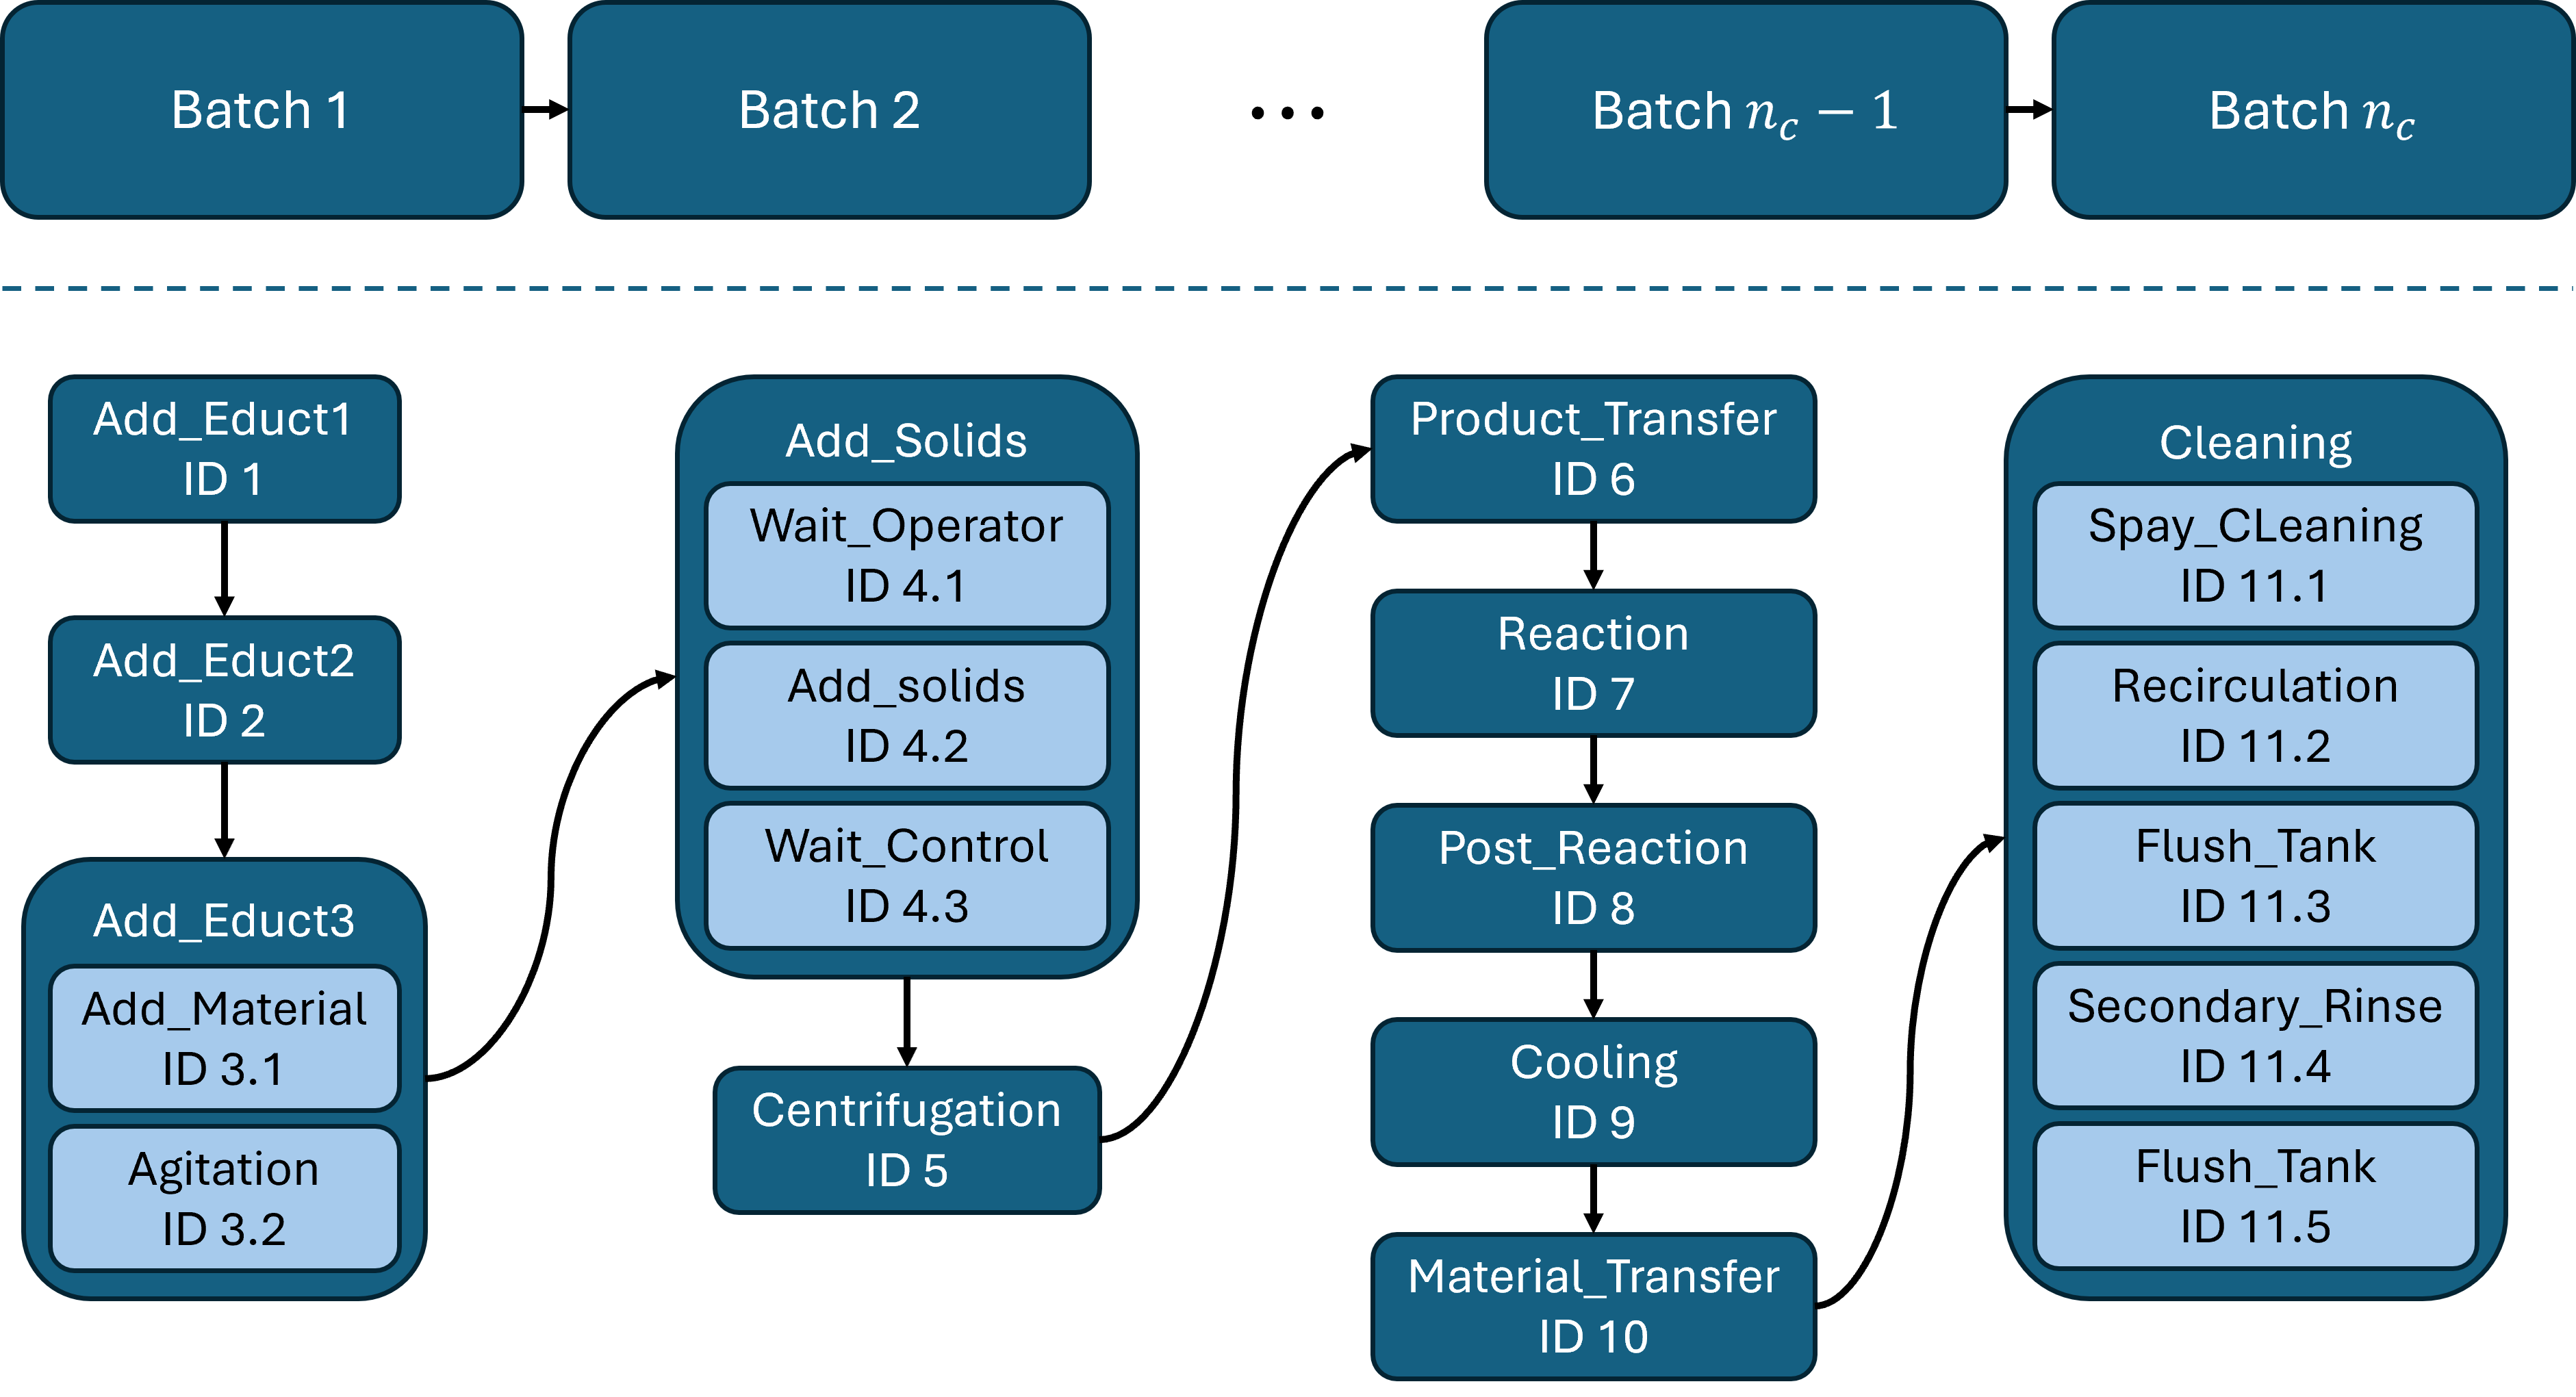
\includegraphics[width=.9\linewidth]{figures/Multiple cycles data/Cycle production layout.png}
    \caption{The structure of a single cycle. A cycle comprises $n_c$ batches that are carried out one by one. Thus, a cycle is simply a collection of a complex task (a batch), that need to be repeated $n_c$ times. The number of times is often based on time or amount of produced drug or substance, such that a cycle is terminated after these criterions are met. We shall later see that in the case of this simulation study, $n_c$ is determined from the accumulated duration of the batches i.e. after a certain amount of time has been simulated, the simulation is terminated. The structure of each batch is observed in the lower part of the figure and consists of $11$ main processes such as addition of solids and chemicals (processes labeled with ID $1$ through $4$). Each process can be made up of a number of \textit{subprocesses} such as the subprocess with ID $4.3$, where the batch waits for a control operator before proceeding.}
    \label{fig:Cycle and process structure}
\end{figure}

For each cycle, we then have a time series, where the ID of the batch is given as well as sensory values. The sensors measure the level of the tank (percentage of mow much of the tank is filled), the height (equivalent to the level), the RPM of a motor that circulates the contents of the tank, the cooling water flow (specifically for the cooling process with ID 9) and the steam flow during the reaction process. We shall however restrict ourselves to only using the level sensor in this thesis but including the other variables could improve on our results later on. We have chosen only the level as it is assumed to be the most descriptive of how much product is eventually produced.

In \autoref{fig:variable description} an example of the temporal evolution of a process is shown (with the previous process as well). We define $T^P_u$ to be the duration of the process/unit operation $u$ and equivalently $M^P_u$ to be the \textit{change} in level during process $u$. Not that we have also defined random variables $T^D_u$ and $M^D_u$. Why we need these will become apparent in \autoref{sec:Data - production processes} but for now we note that they correspond to delays after each of the processes. In particular, after a process is completed, the might be some downtime in the production system due to unforeseen reasons. We shall later see that for some processes, the delays will not influence the level of the tank whereas the reverse is true for other processes such as the reaction (labelled $7$).

\begin{figure}[ht]
    \centering
    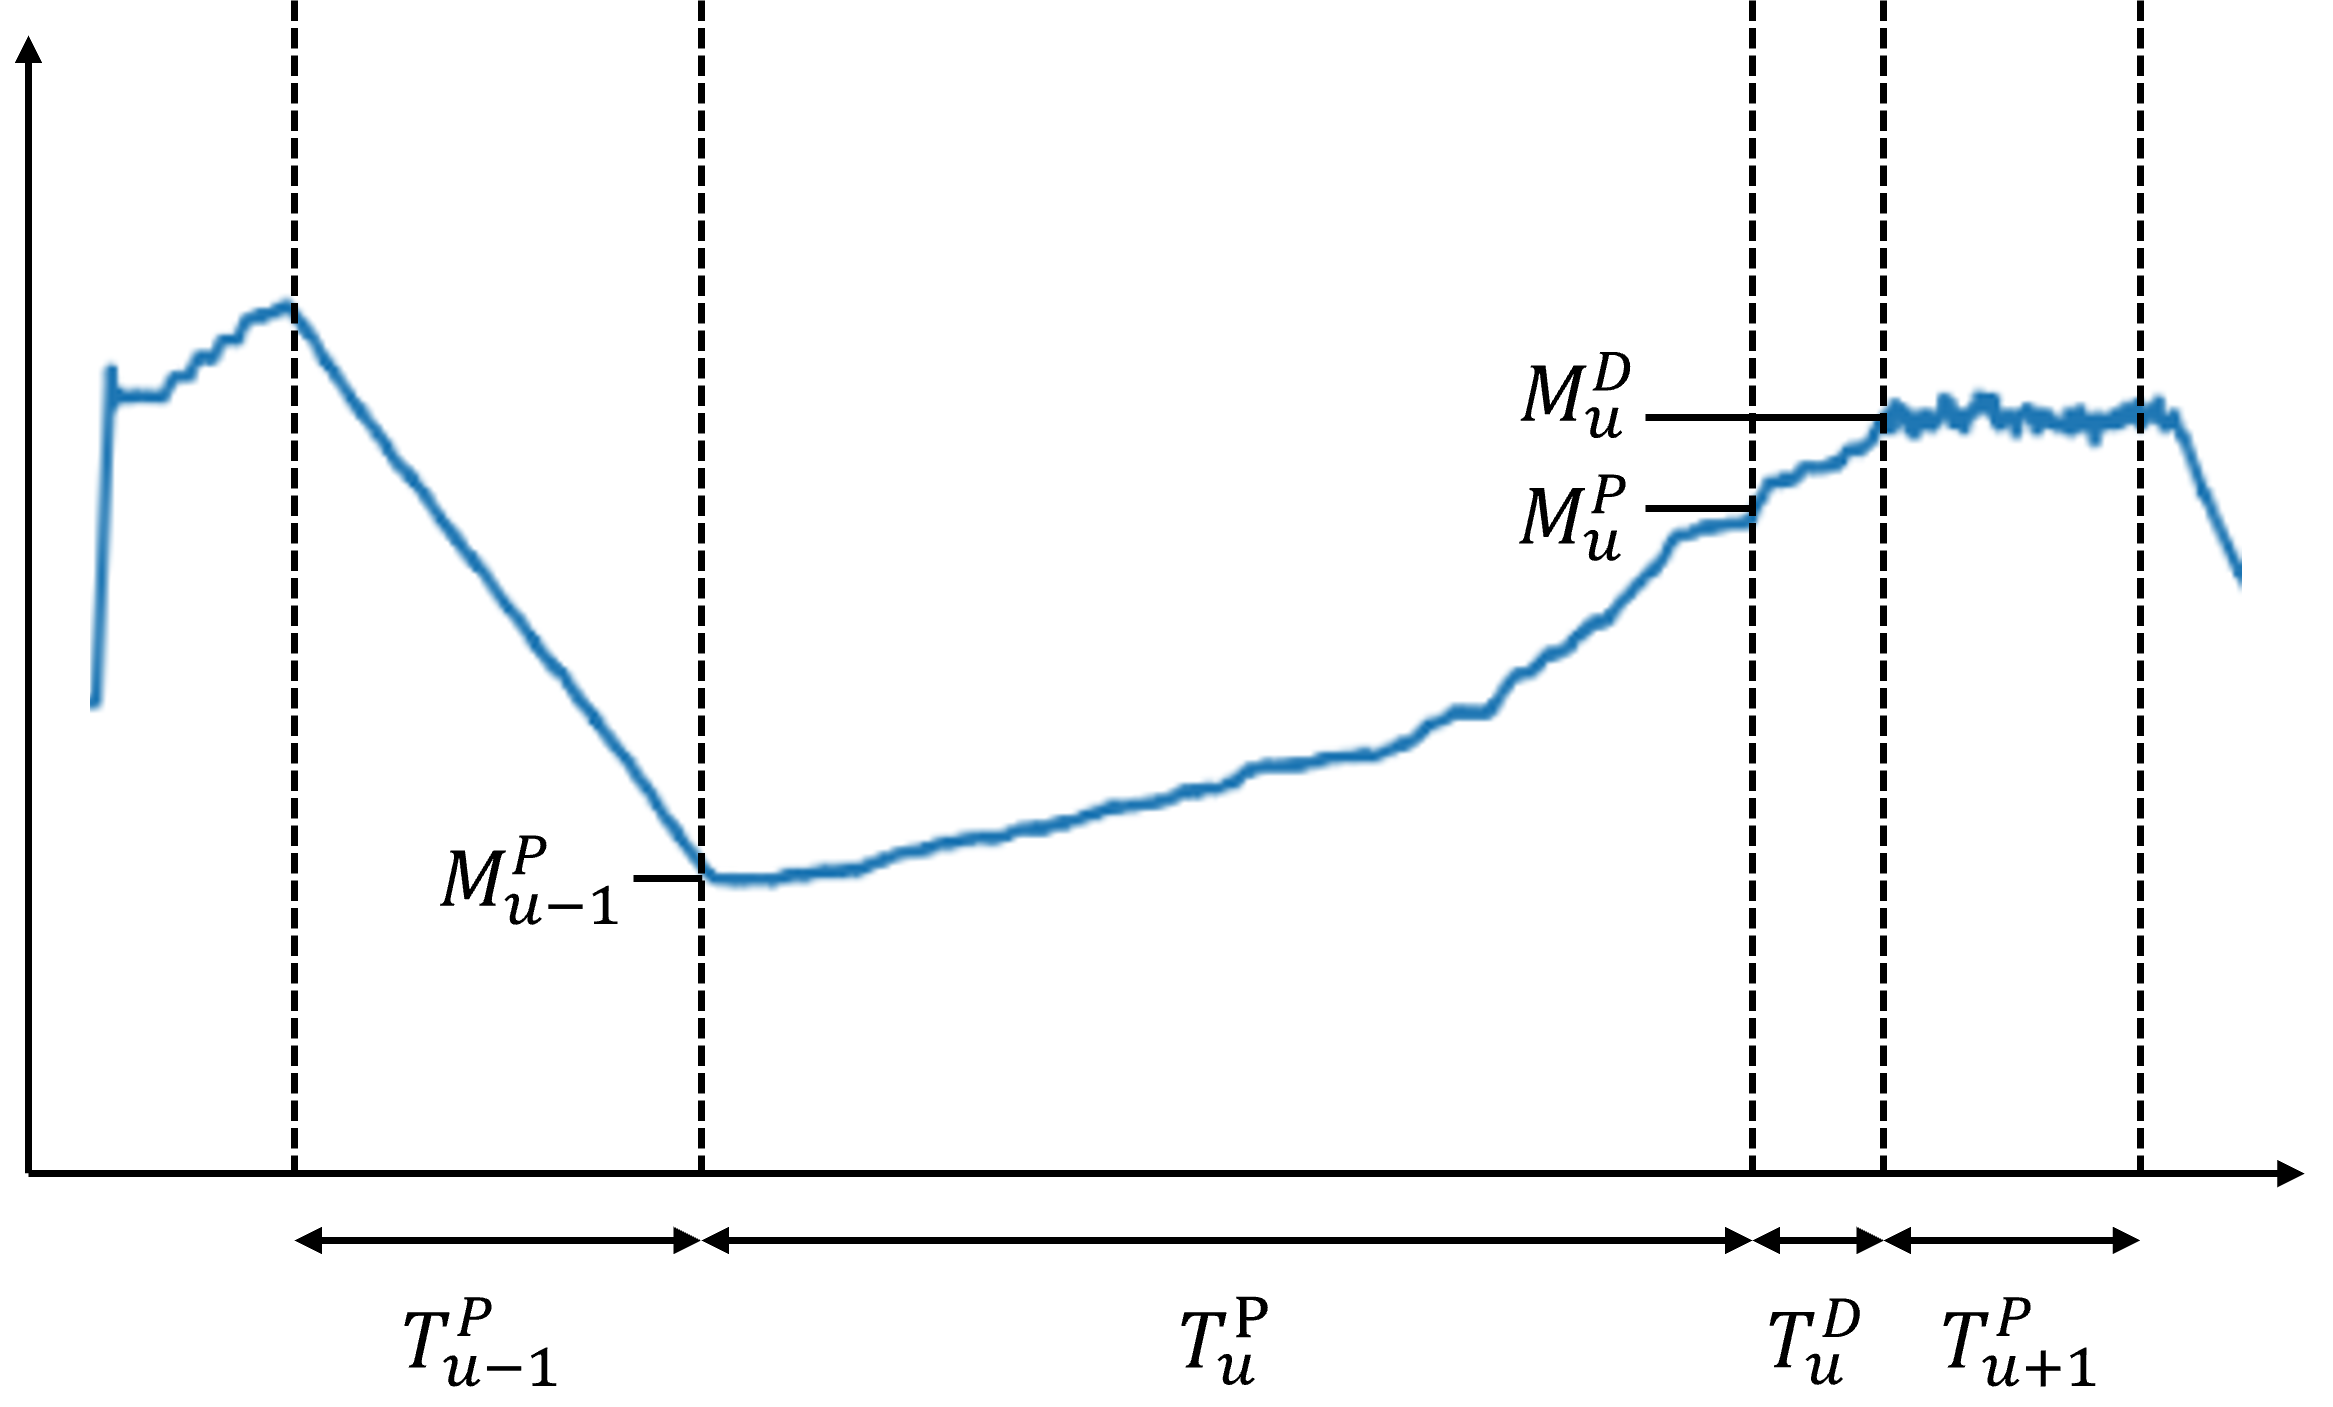
\includegraphics[width=.7\linewidth]{figures/Multiple cycles data/variable desciption.png}
    \caption{Exemplification of the evolution of the level in a tank during a process $u$ and the previous process. The variables $T_u^P$, $T^D_u$, $M_u^P$ and $M^D_u$ related to the process are shown. Note that $M^P_u$ and $M^D_u$ are the changes in level from the previous process or delay of process such that they describe the accumulated evolution in the level of the tank during said process. In particular, changes in levels can occur when the production system is idle.}
    \label{fig:variable description}
\end{figure}

We note that simulations were carried out through a mixture of \texttt{Simulink} and \texttt{Stateflow} simulations. In particular, the continuous subsystems such as the reaction in process $7$ where simulated through \texttt{Simulink} based mass-balance equations.

At this point, we have a rudimentary understanding of how the system is simulated and the meaning of the random variables that are related to each process. We thus continue with some basic statistics concerning the durations of batches. For the remaining of the chapter, we will primarily present results for the duration and delays of the processes as the analysis and results are identical to those of the change in level. Namely, we shall observe that the dimension of the random vector that describes each batch (i.e. durations, delays and level changes) large enough such that no meaningful conclusion on the causal relation between random variables can be drawn. In particular, we will need a framework such as the one presented in \autoref{chap:method}, to discover such relationships.




% The data is chosen as it resembles an actual production data set but is also implemented with what at first glance seem to be fairly realistic variation and noise in measurements. Overall, the point of this example data is to exemplify what one may encounter in a real batch production system and from this try to build a model in order to predict or quantify the behavior of the system or learn hidden (causal) structure important for optimization etc.




% antager senere at der ikke er sammenhæng fra batch til batch. det er måske ok, måske ikke. anyways ser vi hvor godt vi kan forklare processerne udelukkende fra processer i samme batch



% Handler om data, hvorfor det giver mening med baggrund i dette (et mere statistisk udgangspunkt, måske er det ikke altid at man ved hvad der har effekt på hvad, og hvordan det kan kontrolleres)


% the time stamps (in hours) and level in a tank is of the most interest.

% The goal of this section is to describe how different phases of the production covary. 






% We define a set of phases/units $\mathcal{U}$ that each batch consists of. In this case, units are identified with IDs 1 through 10 (with subunits such as 3.1) described further in \autoref{tab:absolute phase ID batch count}. Then, for each unit, we define the random variable $X_u$ to be the total time a batch spends in unit $u$ i.e. the sojourn time related to unit $u$. 


% We also define the random variables $X_u^P$ and $X^D_u$ to be the duration of the actual \textit{processing} and \textit{delay} respectively such that $X_{u} = X_u^P + X_u^D$. It is also important to keep track of the level in the tank after each unit is finished, and we thus define variables $M_u$ and $M^D_u$ to be the level in the tank after unit $u$ and its associated delay respectively. As the units are executed in sequence, as is the case in this data, a simple representation of the variables can easily be visualized and is shown in \autoref{fig:variable description} below.





\section{Basic statistics}
% Initially, we present some basic statistics in  for batches and proceed to discuss the nature of the batches, removing outliers and faulty observations etc.
Before analyzing the time series in more depth and filter out (or correct) troublesome data points, we present some initial statistics on the duration of batches for each cycle. The statistics are summarized in \autoref{tab:cycle basic stats} below. We note that some difference is observed from cycle to cycle, but we choose to assume that these differences are simply a feature of the production system, such that later on, we can combine all observations across all cycles into a single dataset to be used for causal discovery.

\begin{table}[h]
    \centering
    \begin{tabular}{c|c|c|c|c|c}
        Cycle & \makecell{number of                                    \\ batches} & \makecell{mean} & \makecell{variance} & \makecell{standard\\ deviation} & \makecell{coefficient \\ of variation} \\ \hline
        A     & 66                  & 14.776 & 3.641 & 1.908 & 0.1291  \\
        B     & 64                  & 15.644 & 3.915 & 1.979 & 0.1265  \\
        C     & 61                  & 17.714 & 2.330 & 1.526 & 0.08617 \\
        D     & 60                  & 18.069 & 6.922 & 2.631 & 0.1456  \\
        E     & 60                  & 18.088 & 9.613 & 3.100 & 0.1714  \\
        F     & 63                  & 17.227 & 7.766 & 2.787 & 0.1618  \\\hline
        \makecell{Combined \\ cycles} & 374               & 16.876        & 7.218                & 2.687                          & 0.1592
    \end{tabular}
    \caption{Basic batch statistics for each cycle and by combining all cycles into a single data set. The average duration of batches across cycles appear similar when taking the variance of the durations into account. We note that later, we wish to estimate the dependency between pairs of random variables whence more observations is better, as always in data science. We do however note that there appears to be a difference between especially the first three cycles and the latter ones. In particular, the variance is larger for cycles named $D$, $E$ and $F$. The source of this variation is at this point unknown however it could be seen as a feature of the dataset. Namely, if the observations are truly from the same production system, this variation could be an inherent feature of the production system which we should not remove. }
    \label{tab:cycle basic stats}
\end{table}

In the following section, we discuss a problem with some of the batches. Namely, the trailing batches, which appear to be cut-off during simulation. In this way, we shall end up with a total of 368 batches, which after some correction (see \autoref{sec:Data - production processes}) will be our final data set.




% Each batch comprises several states. These include adding materials (IDs 1 through 4), centrifugation (ID 5), product transfer (the precipitate generated from the centrifugation, ID 6), chemical reaction (ID 7), a post operation state (\textcolor{red}{Probably to let it cool down to a point where it is ready for further processing}, ID 8), Cooling of the product (ID 9), material transfer (transfer the gained product before cleaning of the reaction vessel and/or prepare for the next reaction batch, ID 10). Notice that there is a total of 374 batches throughout the 6 observed cycles.



\section{Incompleteness of trailing batches}
In this section, we shall investigate the combined dataset of $374$ batches in more detail. In particular, we shall observe some deviation from \autoref{fig:Cycle and process structure} in terms of labels of each event in the time series and how we have handled these discrepancies. Namely, by looking through the time series for each cycle, we observe entries labeled with negative processes. These, we will investigate the next section and note that from paper introducing the simulations we present here \cite{benchmark-model-to-generate-batch-process-data}, it is by design that some labels are incorrect. Their argument for this is in relation to training a robust machine learning algorithm but as this is none of our concern, we shall manually handle these in correct labels. In particular, the negative labels are initially negated to be positive instead. Hence, we observe events labeled $3$, which is not originally a part of the production system description from \autoref{fig:Cycle and process structure}. With these negative labels transformed, we count for each of the (new) process labels, how many batches are observed. E.g. how many batches are at some point observed to be undergoing process $1$ (the addition of a material). We do this to make sure that in fact every batch go through all processes from \autoref{fig:Cycle and process structure}. The result of this counting batches is presented in \autoref{tab:absolute phase ID batch count}, where the description of the recognized processes has been copied from \cite{benchmark-model-to-generate-batch-process-data}. Note that \texttt{Educt1}, \texttt{Educt2} and \texttt{Educt3} are just some (unknown) materials that we do not care about.
\begin{table}[ht]
    \centering
    \begin{tabular}{c|c|c}
        ID   & Count & Description                                     \\\hline
        1.0  & 374   & Addition of liquid raw material \texttt{Educt1} \\
        2.0  & 374   & Addition of liquid raw material \texttt{Educt2} \\
        3.0  & 181   &                                                 \\
        3.1  & 374   & Addition of liquid raw material \texttt{Educt3} \\
        3.2  & 374   & Agitation                                       \\
        4.0  & 163   &                                                 \\
        4.1  & 374   & Waiting for field operation                     \\
        4.2  & 374   & Addition of solids                              \\
        4.3  & 374   & Waiting for control operator                    \\
        5.0  & 374   & centrifugation                                  \\
        6.0  & 374   & Product transfer                                \\
        7.0  & 370   & Reaction                                        \\
        8.0  & 369   & Post reaction                                   \\
        9.0  & 369   & Cooling                                         \\
        10.0 & 368   & Material transfer
    \end{tabular}
    \caption{The number of batches across all cycles that contains at least one observation for each different process label.}
    \label{tab:absolute phase ID batch count}
\end{table}
Note that we have not included labels pertaining the cleaning operation as these will be handled separately in \autoref{sec:Data - Cleaning operations} where we also argue why we will not use these observations in the later analysis.



% As it may be of interest to investigate the correlation structure of different metrics and variables later on, it is important to understand how each of the batches across the cycles behave. Initially, when looking through the dataset, we observe a few negative phase IDs which will need investigation. However, before we do so, we check that each of the batches actually go through all the states mentioned in \cite{benchmark-model-to-generate-batch-process-data}. 

% Thus, we take the absolute value of the negative phase IDs to ease the analysis prior to the analysis of the negative phase IDs. After this is done, we observe that not all batches go through all the phases and that some seem to have extra phases not described by \cite{benchmark-model-to-generate-batch-process-data}. Namely, from \autoref{tab:absolute phase ID batch count}, we see that IDs 3 and 4 (which are not described in \cite{benchmark-model-to-generate-batch-process-data}) have significantly fewer batches going through this phase. But perhaps even more interesting is the final 4 phases where almost all batches goes through these phases.

Interestingly, the \textit{unrecognized} process labels $3$ and $4$ only occur for processes with subprocesses. We shall later observe that these labels all originate from negative process labels and that they actually correspond to delays between processes as portrayed in \autoref{fig:variable description}. For now, we however concentrate on the last four process labels $7$, $8$, $9$ and $10$. In particular, as all the other process labels (excluding $3$ and $4$) appear exactly $374$ (the number of batches in total) times, we suspect that something weird is going on with these \textit{missing} observations. As hinted to before, it turns out that the simulations have been cut off after $1100$ hours. Therefore, the trailing batch of each cycle does not complete all processes. For example, in \autoref{fig:last batch example}, we have shown the first batch of cycle A as well as the trailing batch and how the over time switch between process labels (not that for this plot, we have not negated the negative process labels)

\begin{figure}[h]
    \centering
    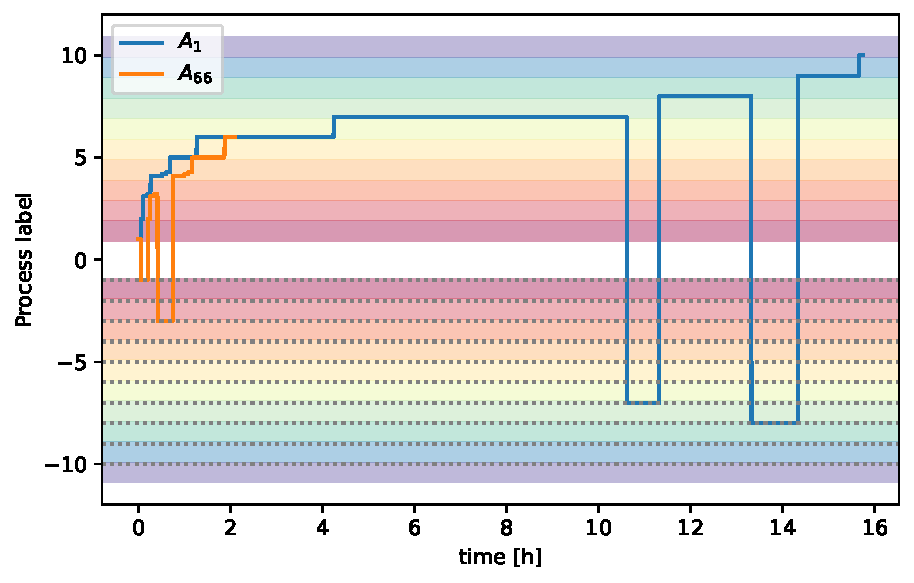
\includegraphics[width=0.75\linewidth]{figures/Multiple cycles data/tailing batch short.pdf}
    \caption{The first and last batch from cycle A. The horizontal colored bars corresponds to the different process labels such that time stamps labeled e.g. $3.1$ and $3.2$ fall in the same colored region. It is clear that the final batch is cut-off before finishing the last process. Furthermore, we observe that the negative process labels for these two batches only occur before the process label enters a new colored region. This hints to the negative process labels are actually delays between processes.}
    \label{fig:last batch example}
\end{figure}

From the above, it is clear that we need to remove the final batches of each cycle. Thus, we now have a total of $368$ batches. In the following section, we shall see in more detail when the negative process labels occur and make the assumption that they correspond to delays between processes. Note that the cleaning operation is not considered in the following section.






\section{Production processes}\label{sec:Data - production processes}
We now focus on the processes labelled $1$ through $10$ from \autoref{fig:Cycle and process structure}. In particular, we shall denote these processes as \textit{production} processes, as they are exactly the processes where a substance is produced or handled in some other way. Initially, we shall however focus on the first processes up to and including $4.3$. Namely, from \autoref{tab:absolute phase ID batch count}, we saw that it was these few initial processes where labels seemed to be weird.

In \autoref{fig:B_22 phase 1-4}, we have shown the \nth{22} batch of cycle B. Once again, we observe the negative process label. We notice that it is only visited once, and only at the of the process which its label corresponds to.

\begin{figure}[h]
    \centering
    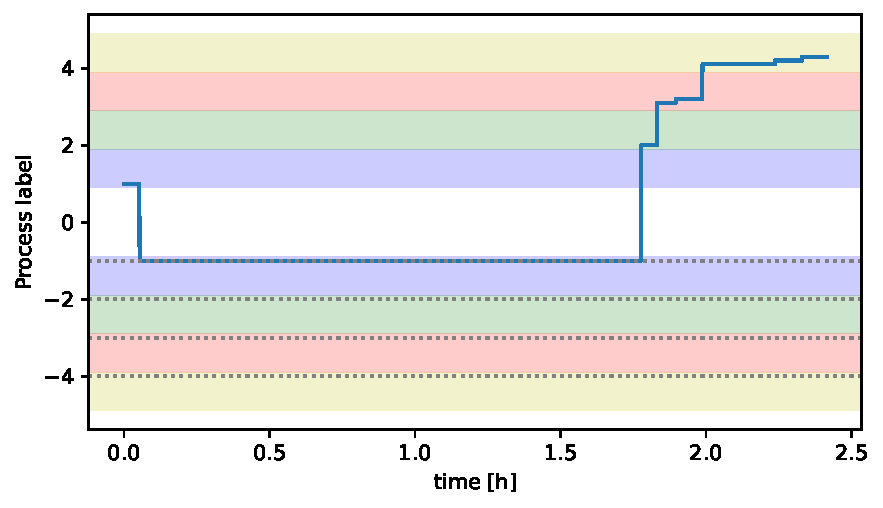
\includegraphics[width=.83\linewidth]{figures/Multiple cycles data/Adding of solids/B_22 long waiting.pdf}
    \caption{The temporal evolution of process labels for batch 22 from cycle B. Only the processes pertaining to the first boxes of \autoref{fig:Cycle and process structure} are shown to easier tell what is happening.}
    \label{fig:B_22 phase 1-4}
\end{figure}

% This part of the process corresponds to events tagged with ID 1 through 10 but will initially concern itself with ID 1 through 4 as much can be learned from the data set here. In \autoref{fig:B_22 phase 1-4} an example of how the process evolves over time through the different phases is shown. Immediately, we observe something weird, namely the negative event IDs.

Continuing the investigating, we see that negative process labels occur throughout all the six cycles. Furthermore, by saving what negative process labels have occurred for each cycle, we obtain \autoref{tab:phase negative observations} where we observe a clear tendency regarding the process labels $-4.1$, $-4.2$ and $-4.3$. Namely, they only occur in cycle F. From \cite{benchmark-model-to-generate-batch-process-data}, we note that cycle F is the only phase containing wrongly labeled time points. In particular, we can conclude that the negative process labels apart from $-4.1$, $-4.2$ and $-4.3$ are not an error in the data set.

\begin{table}[h]
    \centering
    \begin{tabular}{c|c|c|c|c|c|c}
        \diagbox{Event}{Cycle} & A                    & B                    & C                    & D                    & E                    & F                    \\\hline
        -1                     & \cellcolor{black!50} & \cellcolor{black!50} & \cellcolor{black!50} & \cellcolor{black!50} &                      &                      \\\hline
        -2                     &                      &                      &                      & \cellcolor{black!50} & \cellcolor{black!50} & \cellcolor{black!50} \\\hline
        -3                     & \cellcolor{black!50} &                      & \cellcolor{black!50} & \cellcolor{black!50} & \cellcolor{black!50} & \cellcolor{black!50} \\\hline
        -4                     &                      & \cellcolor{black!50} & \cellcolor{black!50} & \cellcolor{black!50} & \cellcolor{black!50} &                      \\\hline
        -4.1                   &                      &                      &                      &                      &                      & \cellcolor{black!50} \\\hline
        -4.2                   &                      &                      &                      &                      &                      & \cellcolor{black!50} \\\hline
        -4.3                   &                      &                      &                      &                      &                      & \cellcolor{black!50} \\\hline
        -5                     & \cellcolor{black!50} & \cellcolor{black!50} & \cellcolor{black!50} & \cellcolor{black!50} & \cellcolor{black!50} & \cellcolor{black!50} \\\hline
        -6                     &                      & \cellcolor{black!50} & \cellcolor{black!50} & \cellcolor{black!50} & \cellcolor{black!50} & \cellcolor{black!50} \\\hline
        -7                     & \cellcolor{black!50} &                      & \cellcolor{black!50} & \cellcolor{black!50} & \cellcolor{black!50} & \cellcolor{black!50} \\\hline
        -8                     & \cellcolor{black!50} &                      & \cellcolor{black!50} & \cellcolor{black!50} & \cellcolor{black!50} & \cellcolor{black!50} \\\hline
        -9                     &                      &                      &                      & \cellcolor{black!50} & \cellcolor{black!50} & \cellcolor{black!50} \\\hline
        -10                    &                      & \cellcolor{black!50} &                      & \cellcolor{black!50} & \cellcolor{black!50} & \cellcolor{black!50}
    \end{tabular}
    \caption{Occurrences of negative process labels. It is observed that the process labels -4.1, -4.2, -4.3 only occur in cycle F which is known to be the only cycle with wrongly labelled phases.}
    \label{tab:phase negative observations}
\end{table}

In \autoref{fig:negative 4 batches}, we have shown some of the batches which contain the process labels $-4.1$ etc. We observe that if either of the three process labels are negative, then all of them are and no corresponding positive labels occur. We shall thus assume that whenever $-4.1$, $-4.2$ or $-4.3$ is observed, it is actually just the negated process label. Correcting the data set under this assumption, we then only have negative process labels that are integer which we have summarized in \autoref{tab:phase negative observations mod} below.
\begin{figure}[H]
    \centering
    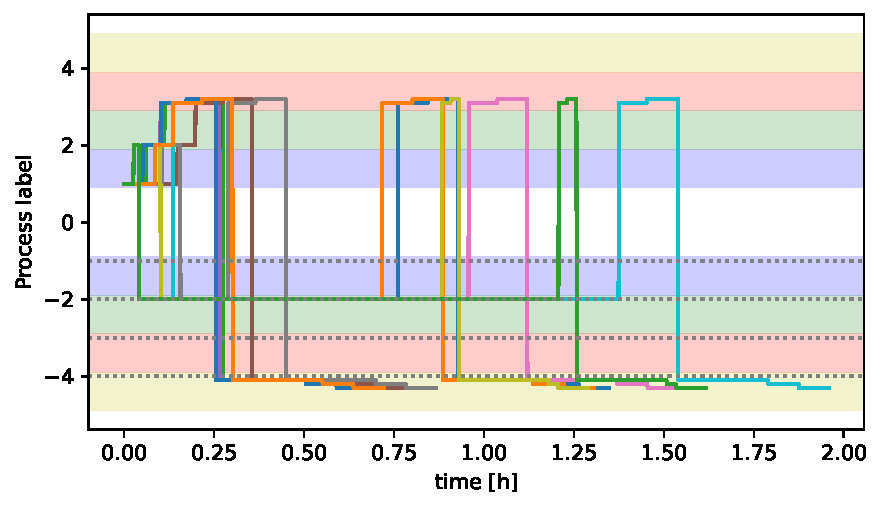
\includegraphics[width=.83\linewidth]{figures/Multiple cycles data/Adding of solids/sample negative sub 4 phases.pdf}
    \caption{13 out of the total 48 batches where at least one of the process labels -4.1, -4.2 or -4.3 were observed.}
    \label{fig:negative 4 batches}
\end{figure}

\begin{table}[H]
    \centering
    \begin{tabular}{c|c|c|c|c|c|c}
        \diagbox{Event}{Cycle} & A                    & B                    & C                    & D                    & E                    & F                    \\\hline
        -1                     & \cellcolor{black!50} & \cellcolor{black!50} & \cellcolor{black!50} & \cellcolor{black!50} &                      &                      \\\hline
        -2                     &                      &                      &                      & \cellcolor{black!50} & \cellcolor{black!50} & \cellcolor{black!50} \\\hline
        -3                     & \cellcolor{black!50} &                      & \cellcolor{black!50} & \cellcolor{black!50} & \cellcolor{black!50} & \cellcolor{black!50} \\\hline
        -4                     &                      & \cellcolor{black!50} & \cellcolor{black!50} & \cellcolor{black!50} & \cellcolor{black!50} &                      \\\hline
        -5                     & \cellcolor{black!50} & \cellcolor{black!50} & \cellcolor{black!50} & \cellcolor{black!50} & \cellcolor{black!50} & \cellcolor{black!50} \\\hline
        -6                     &                      & \cellcolor{black!50} & \cellcolor{black!50} & \cellcolor{black!50} & \cellcolor{black!50} & \cellcolor{black!50} \\\hline
        -7                     & \cellcolor{black!50} &                      & \cellcolor{black!50} & \cellcolor{black!50} & \cellcolor{black!50} & \cellcolor{black!50} \\\hline
        -8                     & \cellcolor{black!50} &                      & \cellcolor{black!50} & \cellcolor{black!50} & \cellcolor{black!50} & \cellcolor{black!50} \\\hline
        -9                     &                      &                      &                      & \cellcolor{black!50} & \cellcolor{black!50} & \cellcolor{black!50} \\\hline
        -10                    &                      & \cellcolor{black!50} &                      & \cellcolor{black!50} & \cellcolor{black!50} & \cellcolor{black!50}
    \end{tabular}
    \caption{In the modified data set, where $-4.1$, $-4.2$ and $-4.3$ have been converted their absolute value. We observe that the occurrence of negative labels is not identical from cycle to cycle. Depending on the parameters of the simulation, this could either be per happenstance on different settings of the simulation. Either way, we assume that as the simulation is based on the same production system, this variation is observed naturally. Hence, we shall not do more with these observations in terms of filtering them out or correcting them.}
    \label{tab:phase negative observations mod}
\end{table}

From \autoref{tab:phase negative observations mod}, we see that cycles $D$, $E$ and $F$ appear to contain more negative process labels. We will however assume that the cycles are simulated from the same production system such that no hyperparameters were changes. In particular, we shall assume that the observations of negative process labels occurs at random, independently of the cycle.

Furthermore, by plotting the different batches from different cycles, it is apparent that the negative process labels always occur after each process (including subprocesses) and before the next process. I.e. we only observe the label $-1$ after $1$ and before $2$. Likewise, $-3$ only occurs after both $3.1$ and $3.2$ but before $4.1$. As hinted to before, we shall thus assume that these negative process labels corresponds to delays between processes. This does make sense from a production point, but they also note in \cite{benchmark-model-to-generate-batch-process-data} that delays between operations have been implemented.



\newpage

At this point, it would seem that the labels of the processes are understood for phases 1 through 10 corresponding to the actual production in each batch. Thus, we proceed by searching relationships and otherwise quantifying the durations of each phase, both delays and duration for each of the phases. As a beginning, histograms for each of the phases and delays are plotted in \autoref{fig:histogram production durations}. Notice that phases 4.1, 4.3 and 8 are not shown, this is because they always last 15 min, 5 min and 2 hours respectively with the only derivation being in machine precision either when loaded or during calculations. Furthermore, notice that for the negative IDs i.e. the delays, the orange bar. This bar represents the cases where no delay was observed which is thus modelled as an atom at 1.

\begin{figure}[H]
    \centering
    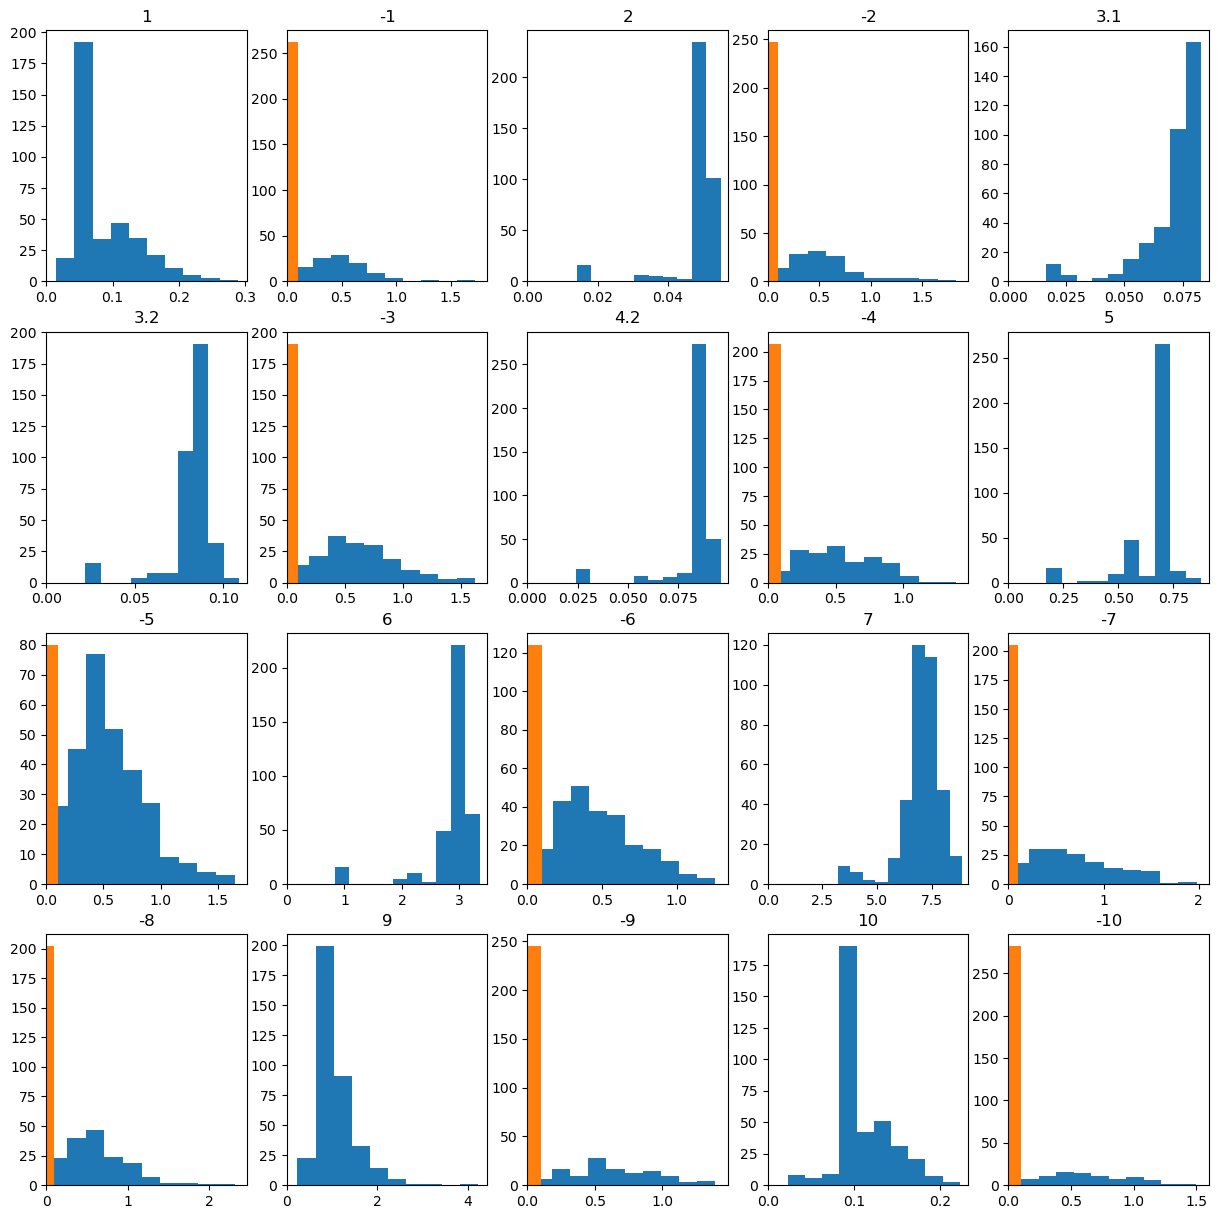
\includegraphics[width=\linewidth]{figures/Multiple cycles data/Adding of solids/hisstograms w atoms.png}
    \caption{Histograms of all phases and delays which are non-constant.}
    \label{fig:histogram production durations}
\end{figure}

Apart from the above comments, not much catches the eye when looking at \autoref{fig:histogram production durations}, and we thus proceed by checking if any correlation is immediately present.

\begin{table}[h]
    \centering
    \begin{tabular}{c|cccccc}
        Cycle                                                 & A       & B       & C       & D      & E      & F      \\\hline
        $\widehat{\mathbb{E}\left[\sum X_u\right]}$           & 13.993  & 13.898  & 15.343  & 14.471 & 14.589 & 14.418 \\\hline
        $\widehat{\text{Var}\left(\sum X_u\right)}$           & 0.95636 & 0.46587 & 0.76111 & 4.9589 & 4.2678 & 5.3545 \\\hline
        $\sum \widehat{\text{Var}\left(X_u\right)}$           & 0.50590 & 0.31182 & 0.36667 & 1.8322 & 1.5788 & 1.9696 \\\hline
        $\widehat{\mathbb{E} \left[\sum X^D_u\right]}$        & 0.96398 & 1.9402  & 2.4503  & 3.6050 & 3.7390 & 3.0041 \\\hline
        $\widehat{ \text{Var} \left(\sum X^D_u\right)}$       & 0.31843 & 0.39117 & 0.90187 & 1.2468 & 1.2787 & 1.0462 \\\hline
        $\sum \widehat{\text{Var}\left(X^D_u\right)}$         & 0.34921 & 0.53198 & 0.74914 & 1.4357 & 1.2454 & 1.3099 \\\hline
        $\widehat{\mathbb{E} \left[\sum X_u \, X^D_u\right]}$ & 1.9321  & 1.5001  & 4.8191  & 6.4225 & 6.0405 & 6.3343 \\\hline
        $\widehat{\text{Var} \left(\sum X_u \, X^D_u\right)}$ & 3.7798  & 0.89920 & 16.870  & 22.133 & 12.660 & 16.194
    \end{tabular}
    \caption{Each of the time related variables $X_i$ and $D_i$ and variance description.}
    \label{tab:data variation and covariance}
\end{table}


\subsection{Correlations}

Lige en korrelationsmatrix
\begin{figure}[H]
    \centering
    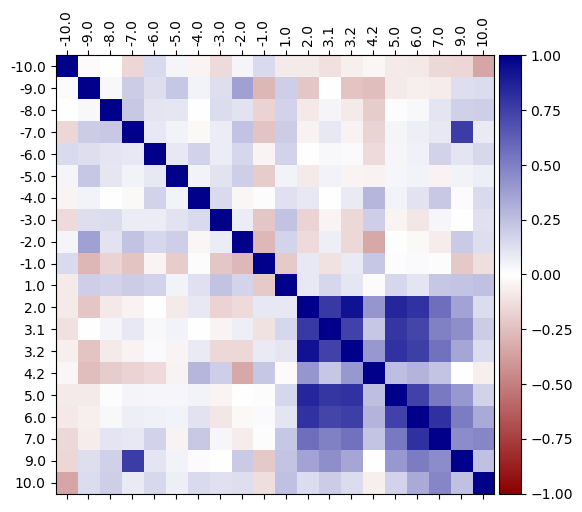
\includegraphics[width=.9\linewidth]{figures/Multiple cycles data/Correlation matrix production and delays.png}
    \caption{Correlation matrix for all phases with non-constant duration.}
\end{figure}

9 og 10 er ikke specielt korreleret med noget (afkøling og materiale overførsel). Ellers er 2 fremt il og med reaktionen alle korrelerede med hinanden. Eftersom rent fysisk det udvikles i tid, må handlingen i 2 påvirke de næste osv.

\begin{figure}
    \centering
    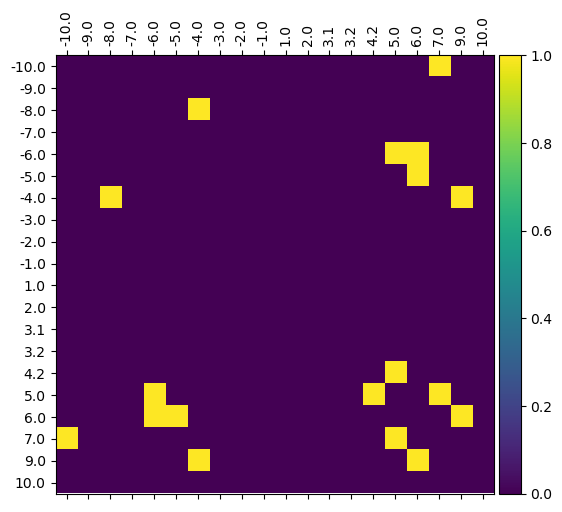
\includegraphics[width=.9\linewidth]{figures/Multiple cycles data/Permutation test rho 10 mil.png}
    \caption{Permuteringstest med $\alpha = 0.05$. Also run with less simulations but same result at 1 mil and 10k sims. The Benjamin-Hochberg procedure on the upper (or lower) triangle reveals that none of the correlations are significant.}
\end{figure}

Umiddelbart lidt spøjst hvis delay på 7 (reaktion) skulle have noget med tiden for afkøling at gøre, især at den skulle være positiv (ville man ikke tro delay efter produktion ville afkøle mere og dermed reducere behov for afkøling, medmindre varmt steam bliver tilføjet også under delay på 7)




Herunder er samme korrelationsmatrix, dog hvor delay og phasens varighed lagt sammen (også med sub phases såsom 3.1, 3.2 og -3 tilsammen bliver 3)

\begin{figure}[H]
    \centering
    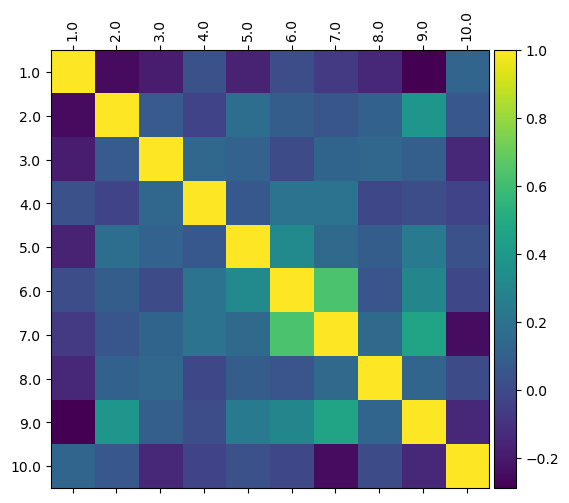
\includegraphics[width=.7\linewidth]{figures/Multiple cycles data/Correlation matrix collapsed phases.png}
    \caption{Correlation matrix for all phases collapsed}
\end{figure}


Ligeledes scatter plots for superdiagonalen i ovenstående matrix. Altså phase 1 overfor phase 2, phase 2 overfor phase 3 osv. Er farvelagt efter hvilken cycle de kommer fra. \autoref{tab:phase negative observations mod} forklarer hvorfor nogle af de horisontale fremkommer sammen med \autoref{fig:histogram production durations} (selve produktionstiden er ret kort sammenlignet med delay.)
\begin{figure}[H]
    \centering
    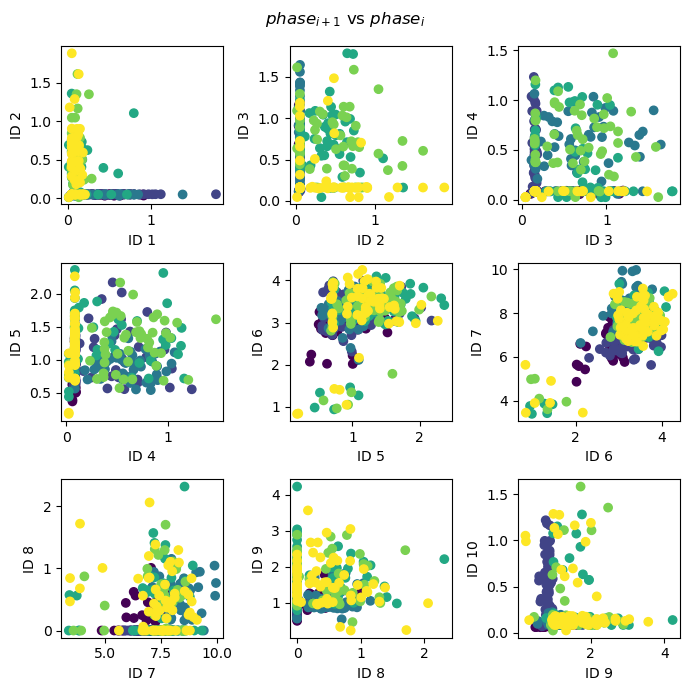
\includegraphics[width=\linewidth]{figures/Multiple cycles data/phase scatter vs next phase.png}
    \caption{Phases vs their next phase when collecting everything regarding a single phase into a total time duration}
\end{figure}



% Check at eventID altid er kronologisk stigende, absolut værdi (med undtagelse for 3 og 4, der gør lidt tilbage grundet waiting time)

% Peaks i e.g. 1, kommer det fra en specifik cycle?

% sammenhæng med fyldningsniveau?

% correlaiton diagrammer

% Betyder delay på 7 (ID -7) at der bliver produceret mere? Eller er det bare den er færdig og man så venter til næste operation?

% Skal man måske prøve at modellere sig ud af korrelationen? Måske ved at kigge på fyldningsniveauet, da det nok beskriver en del


\newpage
\section{Cleaning operations}\label{sec:Data - Cleaning operations}
Sometimes, the vessel is cleansed. This is however not every time after a batch so might be interesting to investigate further. Initially, per cycle, the cleanings are summarized in the following table with basic statistics. As can be seen, there is quite some differences.

The most notifiable differences per batch are the number of cleanses especially when comparing to \autoref{tab:cycle basic stats}. For the first two cycles, the cleanses seem to be in between every batch, which is indeed also the while the later four are only sometimes. Furthermore, although the cleanses are between every batch for cycles A and B, the variances are extremely different. For the last four cycles, they seem to be grouped further, E and F are very alike while cleanses in C and D are generally longer although D has a substantially smaller variance than C.

\begin{table}[h]
    \centering
    \begin{tabular}{c|c|c|c|c|c|c|c}
        Cycle & \#ops & min   & max   & $\mu$ & $\sigma^2$ & $\sigma$ & $\sigma / \mu$ \\ \hline
        A     & 65    & 1.113 & 3.067 & 1.917 & 0.269      & 0.518    & 0.270          \\
        B     & 63    & 1.324 & 1.751 & 1.566 & 0.00883    & 0.0939   & 0.0600         \\
        C     & 9     & 1.544 & 3.306 & 2.153 & 0.277      & 0.526    & 0.245          \\
        D     & 10    & 1.474 & 2.009 & 1.581 & 0.0212     & 0.146    & 0.0922         \\
        E     & 10    & 0.827 & 1.584 & 1.465 & 0.0462     & 0.215    & 0.147          \\
        F     & 10    & 0.748 & 1.610 & 1.466 & 0.0595     & 0.244    & 0.166
    \end{tabular}
    \caption{Per cycle cleansing statistics}
    \label{tab:cycle cleansing stats stats}
\end{table}



To verify these observations and potentially discovering more important facts of their probability distributions, histograms are plotted in the following \autoref{fig:cycle cleaning histograms}. We indeed again observe the likeliness between the cycles A and B, C and D, E and F respectively. Also, for the first two cycles and more so cycle B, the cleaning times are somewhat normally distributed although cycle A has a very heavy right tail in that case. The later four cycles only have 10 observations but the mode (i.e. peak) seem to be about the same.

\begin{figure}[h]
    \centering
    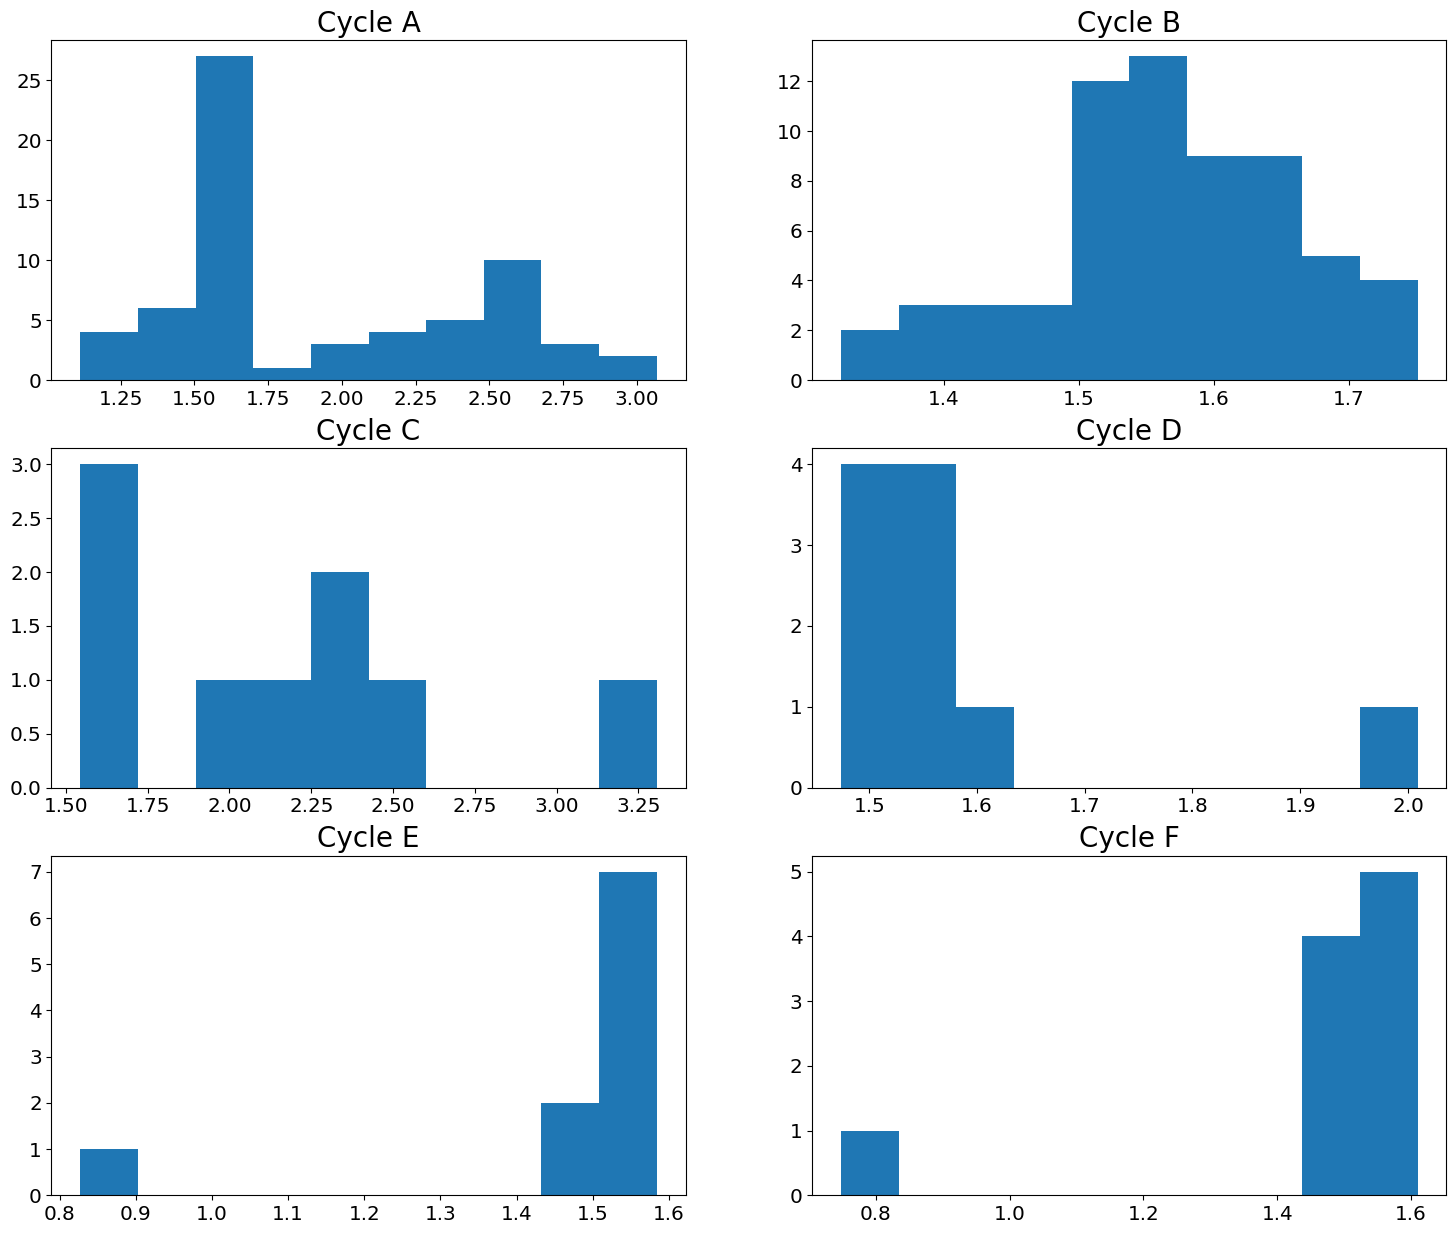
\includegraphics[width=0.8\linewidth]{figures/Multiple cycles data/Cleaning batches histograms.png}
    \caption{Each of the 6 cycles, cleaning operations histograms.}
    \label{fig:cycle cleaning histograms}
\end{figure}

From the above observation of like modes one may want to observe the histogram of the combined set of cleaning times. In particular, under the hypothesis that the durations are actually from the same probability distributions and realized independently within each cycle a histogram of all the observations are of interest and is shown in \autoref{fig:cycle cleaning histograms combined} below.


\begin{figure}[H]
    \centering
    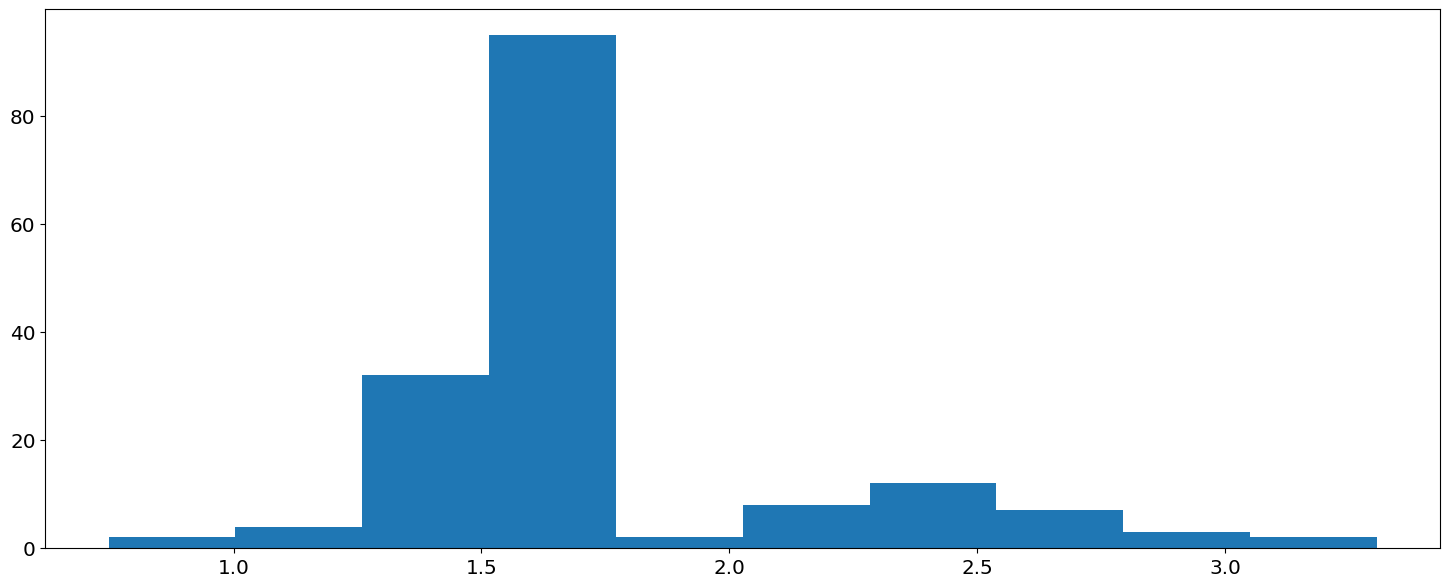
\includegraphics[width=0.8\linewidth]{figures/Multiple cycles data/Cleaning batches histograms combined.png}
    \caption{Combined cleaning operations histograms.}
    \label{fig:cycle cleaning histograms combined}
\end{figure}


Finally, to get a better overview of the irregularities is the number of cleaning periods (mostly concerning cycles C through F), each cleaning operation is shown in the following \autoref{fig:cycle cleaning time series}. The vertical shaded rectangles signify the period in which a cleaning operation is taking place. Furthermore, the event IDs are shown but to get a clearer view on what is going on, a single rectangle (zoomed in) is shown in \autoref{fig:cycle cleaning time series single}.

\begin{figure}[H]
    \centering
    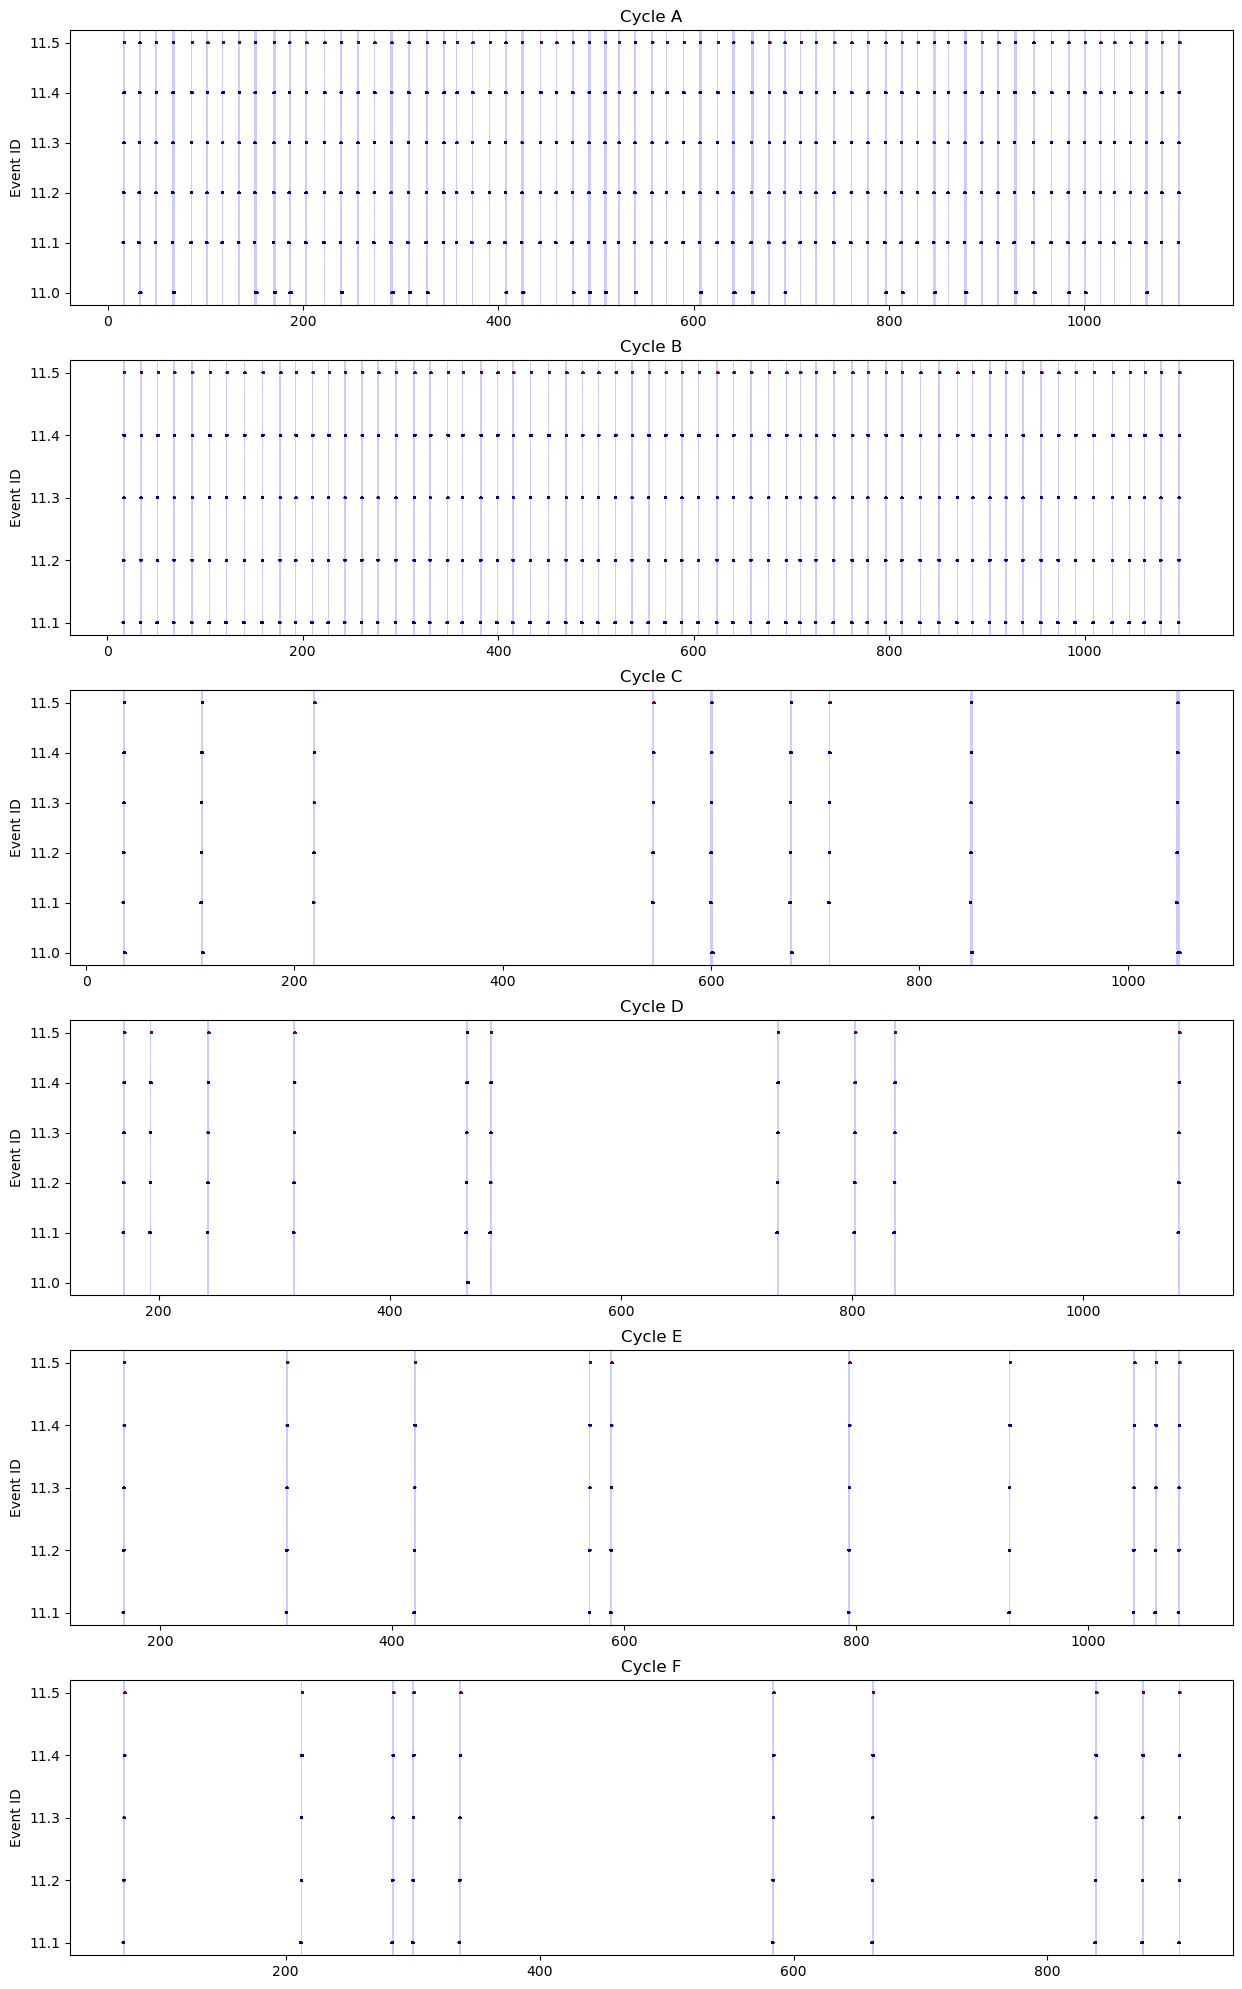
\includegraphics[width=0.9\linewidth]{figures/Multiple cycles data/Cleaning batches.png}
    \caption{Each of the 6 cycles, cleaning (corresponding to \texttt{BatchID = 0}). Each \textit(Cleaning Procedure), CIP, is highlighted with an opaque interval (the blue rectangles). The dots marked with red (only ID 11.5, but not all of these are red), is if the Cleaning ID is 0.}
    \label{fig:cycle cleaning time series}
\end{figure}


\begin{figure}[h]
    \centering
    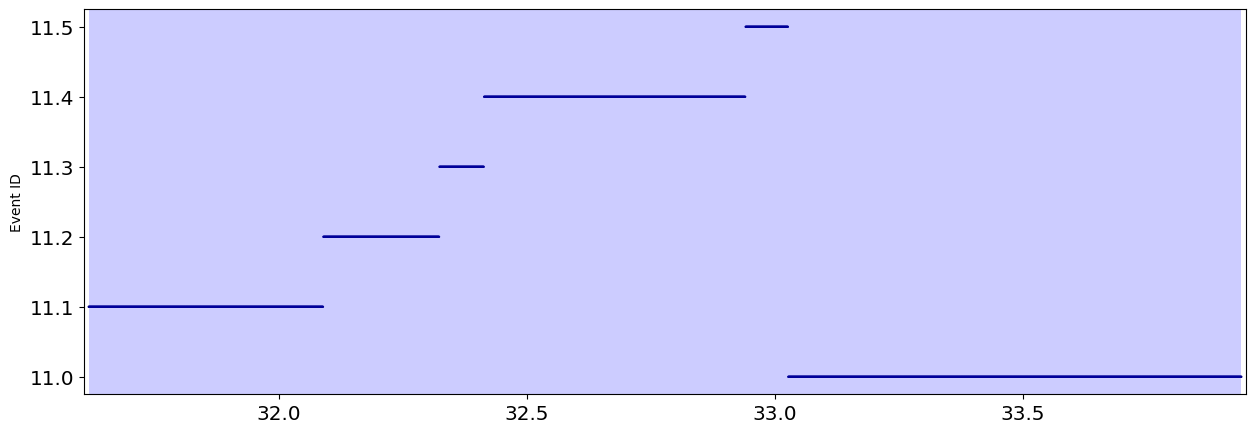
\includegraphics[width=0.9\linewidth]{figures/Multiple cycles data/Cleaning batches timeseries single.png}
    \caption{A single blue rectangle zoomed in}
    \label{fig:cycle cleaning time series single}
\end{figure}

It is observed that the observations marked with red in figure \ref{fig:cycle cleaning time series} occur exactly when that specific cleaning operation does not go to the state 11.0 after the flush of the tank (event ID 11.5) and vice versa. It is hard to conclude what this may mean, but the cleaning being in state 11.0 may indicate that the system is idle before continuing the next batch like what is observed from the other steps of the process flow. Also, it is noted that while the red dots occur nothing else is happening according to the dataset.


From a modelling point of view, the cycles C through F can be thought of as the cleansing operation having a probability of not happening or equivalently as having a duration of 0. It is thus of interest to observe what the probability of cleaning after an operation is. From \autoref{tab:cycle basic stats} and \autoref{tab:cycle cleansing stats stats}, we that indeed for cycles A and B, the probability is 100 \% when disregarding the possibility of cleaning after the final batch. Hence, we see that for the remaining cycles, the probabilities of cleaning the tank after an operation are as in \autoref {tab:cycle cleaning prob}

\begin{table}[h]
    \centering
    \begin{tabular}{c|r}
        Cycle & \% cleaning \\ \hline
        A     & 100.00      \\
        B     & 100.00      \\
        C     & 15.00       \\
        D     & 16.95       \\
        E     & 16.95       \\
        F     & 16.13
    \end{tabular}
    \caption{Per cycle probability of cleaning}
    \label{tab:cycle cleaning prob}
\end{table}


Furthermore, let $C_i$ denote whether the $i$th batch is followed by a cleaning of the tank or not. It is then of interest if the next batch is followed by a cleaning given whether the current batch is followed by a cleaning. In particular, we count for each of the cycles the transitions which are shown in the following tables. Notice that the number of observations is two less than the total number of batches within each specific cycle. This is due to the last batch is never followed by a cleaning (nor is the first batch superseded by a cleaning procedure) which results in one less observation and also due to the fact that we are logging transitions and hence lose another observation. To test for randomness, a Chi-squared test is carried out on each of the cycles to check for independence. It is observed all the cycles exhibit independence between the groups i.e. there is no statistical evidence for information is gained about if the next batch is followed by a cleaning operation given whether the current batch is followed by a cleaning operation.

\begin{table}[h]
    \begin{subtable}{.5\linewidth}
        \centering
        \begin{tabular}{c|c c}
            \diagbox{$C_i$}{$C_{i+1}$} & No & Yes \\ \hline
            No                         & 41 & 9   \\
            Yes                        & 9  & 0
        \end{tabular}
        \caption{C, $p=0.3293$}
        \label{tab:cycle C Contingency table}
    \end{subtable}%
    \begin{subtable}{.5\linewidth}
        \centering
        \begin{tabular}{c|c c}
            \diagbox{$C_i$}{$C_{i+1}$} & No & Yes \\ \hline
            No                         & 41 & 8   \\
            Yes                        & 7  & 2
        \end{tabular}
        \caption{D, $p=0.6456$}
        \label{tab:cycle D Contingency table}
    \end{subtable}
    \begin{subtable}{.5\linewidth}
        \centering
        \begin{tabular}{c|c c}
            \diagbox{$C_i$}{$C_{i+1}$} & No & Yes \\ \hline
            No                         & 41 & 7   \\
            Yes                        & 7  & 3
        \end{tabular}
        \caption{E, $p=0.3532$}
        \label{tab:cycle E Contingency table}
    \end{subtable}%
    \begin{subtable}{.5\linewidth}
        \centering
        \begin{tabular}{c|c c}
            \diagbox{$C_i$}{$C_{i+1}$} & No & Yes \\ \hline
            No                         & 41 & 9   \\
            Yes                        & 9  & 1
        \end{tabular}
        \caption{F, $p=1.0000$}
        \label{tab:cycle F Contingency table}
    \end{subtable}

    \caption{Contingency table for Cycle C-F}
    % \label{tab:}
\end{table}

Thus collecting the observations from all the last four cycles, we may want to model the atom of the cleaning procedure independently of the previous batch and with a probability of $0.8375$ corresponding to the cleaning procedure only being carried out $16,25$\% of cases.

Finally, we show the autocorrelation function for each the four cycles C-F in \autoref{fig:cycle cleaning ACF} and note that all the ACF stay within the 95\% confidence interval.

\begin{figure}[h]
    \centering
    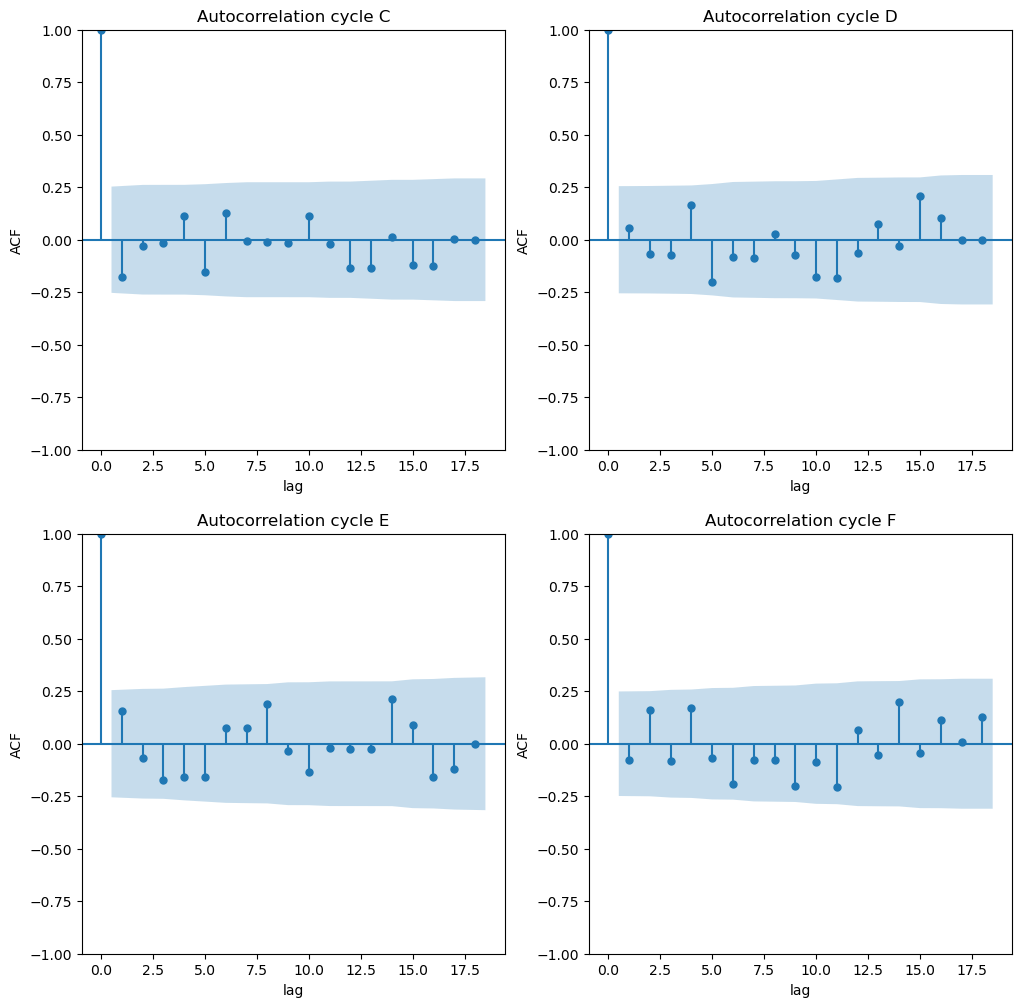
\includegraphics[width=0.8\linewidth]{figures/Multiple cycles data/Cleaning Autocorrelation.png}
    \caption{Autocorrelation function for each of the final 4 cycles. As can also be seen from this there seem to be no information to be gained of $C_i$ from $C_{i-1}$.}
    \label{fig:cycle cleaning ACF}
\end{figure}

\end{document}


% There is a relationship between the red dots and when the cleaning does not \textit{return} to state 11.0 -> probably no


% Correlationssky mellem delay og % filled




% 1 og -1 sammen osv -> ny korrelationsmatrix -> DONE

% Binært billede af korrelationsmatrix om hvad der er med ud fra threshhold T (varirer lidt om hvad der kan give mening -> absolutværdi af korrelation obv.))

% plot tider for operationer over for hinanden: O1 vs O2, O2 vs O3 -> DONE



% Bo skal sende Claras PhD. vedrørende togmodeller

% MODEL: baseret på threshhold for en phase, kan gå to veje, MPH* mmodel i den ene (måske) , MPH* i den anden + hale (eksponentiel)


% CME ILT TELEK

% undersøg delay propagation - artikler


% se på kurver om der sker noget specielt under negative event med fyldningsniveauer